\chapter{Implementação}

{\color{red} 1 Esse capítulo iremos reformula-lo futuramente, vamos deixar pronto o inicio e depois damos continuidade daqui}

{\color{red} Criar um novo chapter de testes a seguir deste}




Para o desenvolvimento do projeto, houveram uma série de reuniões onde o objetivo era delimitar e estabelecer alguns requisitos para a implementação do projeto, que de suma relevância para o andamento e funcionamento dos setores a serem implantados.

Para o desenvolvimento foi estabelecido uma média de 30 dias de implementação direta no desenvolvimento do projeto, considerando que a data prevista para a entrega final do projeto será em 2020/2.

\section{Tecnologias}
Para o desenvolvimento do sistemas, foram divididas em três aplicações: uma visando a parte WEB, outra visando dispositivos móveis com os sistemas Android e IOS e para efetuar a comunicação entre os sistemas e o banco dados, foi elaborado uma aplicação de servidor cujo valida as requisições e efetua a comunicação entre as aplicações visíveis e o banco de dados.

\subsection{Aplicação WEB}

Para o desenvolvimento foi utilizada as tecnologias pré requisitadas pela empresa Duas Rodas, sendo elas HTML5, SCSS e como complemento, utilizamos a biblioteca ReactJS.



{\textbf{HTML5} - É uma linguagem de marcação utilizada para desenvolvimento Web, esta nova versão traz consigo importantes mudanças quanto ao papel do HTML no mundo da Web, através de novas funcionalidades como semântica e acessibilidade.}

{\textbf{SCSS} - É uma folha de estilo interpretada e compilada em Cascading style sheets, ao ser interpretado é criado blocos de códigos de regras CSS. Resumidamente é utilizada para fazer o Design do sistema, com cores personalizadas, etc.}

{\textbf{ReactJs} - O React é uma biblioteca JavaScript de código aberto com foco em criar interfaces de usuário em páginas web.}

\subsection{Aplicação Mobile}
Utilizando as tecnologias Ionic 4 e TypeScript esta aplicação é desenvolvida paralelamente com as demais aplicações, tem como objetivo a mobilidade, facilidade de acesso e interação podendo ser utilizado em qualquer lugar dentro da empresa.

{\textbf{TypeScript} - TypeScript é um superconjunto de JavaScript desenvolvido pela Microsoft que adiciona tipagem e alguns outros recursos a linguagem. É utilizada somente pelos desenvolvedores, pois auxilia na construção do código fonte. Seu código é transpilado para JavaScript, no final das contas tudo escrito em TypeScript vira JavaScript.}

{\textbf{Ionic 4} - O Ionic é um framework open source para desenvolvimento de aplicativos móveis multiplataforma.}

\subsection{Aplicação do Servidor}
A aplicação do servidor é o canal centralizador das demais plataformas. Ela tem acesso único e exclusivo ao banco de dados. É responsável por todas as validações e executa regras de negócio.

\section{Códigos Desenvolvidos} 

Nesta etapa será apresentado alguns trechos dos códigos implementados para ilustrar o funcionamento e o entendimento de partes específicas do código fonte, onde os mesmos contém regras complexas e de suma importância ao leitor.

\subsection{Mapeamento do Banco de Dados com TypeOrm}

A figura \ref{code_server_type-orm} demonstra a utilização da TypeOrm, onde na definição de classe é possível mapear as colunas e relações das tabelas no banco de dados. Na linha 5 temos o nome da tabela do banco de dados, a própria \textit{ORM} se encarrega de mapear a tabela ao criar a mesma. A linha 8 é designado a coluna criada para este \textit{Model}.

\begin{figure}[htb]
	\caption{\label{code_server_type-orm}Mapeamento do Banco de Dados com TypeOrm}
	\begin{center}
		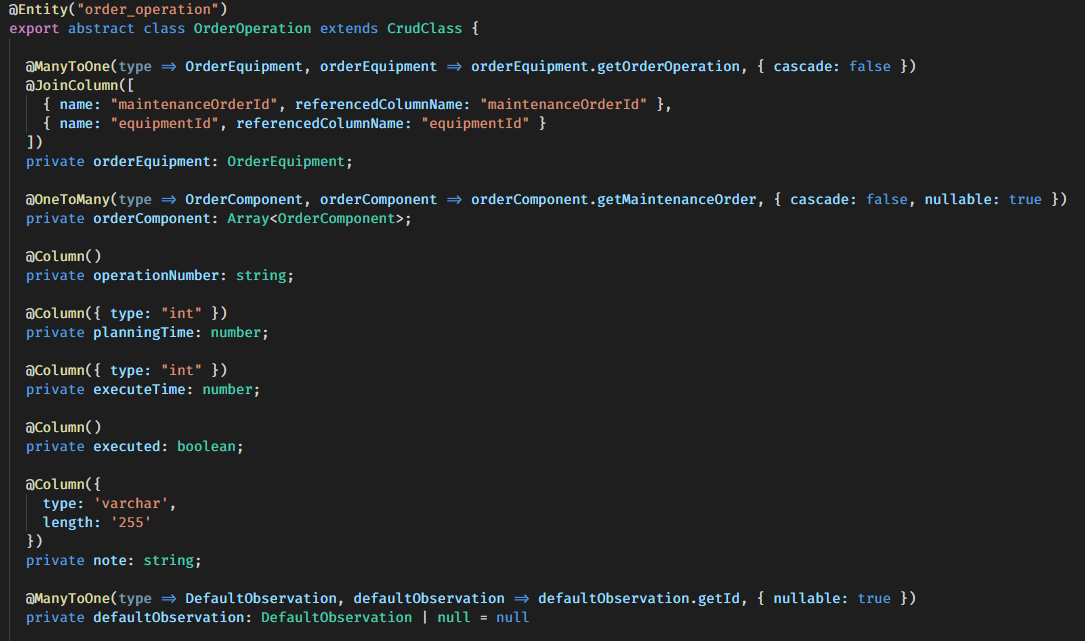
\includegraphics[scale=0.60]{./Figuras/code/server/type-orm.png}
	\end{center}
	\legend{Fonte: os autores (2020)}
\end{figure}

\subsection{Validação de Objetos com o Class Validator}


Na figura \ref{code_server_class-validator} é possível ver o mapeamento de uma classe com o \textit{decorator} ''IsNotEmpty'' na propriedade ''description''. Esse \textit{decorator} irá validar se a propriedade está vazia ou não, caso esteja vazia, irá retornar o erro ``Descrição: Campo obrigatório.'' conforme definição no próprio \textit{decorator}.

\begin{figure}[htb]
	\caption{\label{code_server_class-validator}Validação de Objetos com o Class Validator}
	\begin{center}
		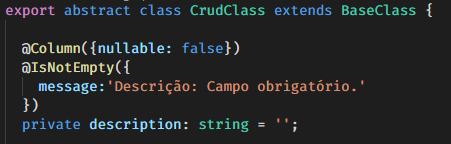
\includegraphics[scale=1.30]{./Figuras/code/server/class-validator.png}
	\end{center}
	\legend{Fonte: os autores (2020)}
\end{figure}





\subsection{Controller: Validação do Objeto Recebido}

Na figura \ref{code_server_class-validator} foi definido uma validação para o campo description. Essa validação implica na obrigatoriedade do campo. Porém, isso não ocorre automaticamente, para a validação de fato funcionar, deve-se executar o método validate da biblioteca \textit{Class Validator}. Na imagem acima, a figura \ref{code_server_class-validator}, demonstra a utlização no código do servidor.

\begin{figure}[htb]
	\caption{\label{code_server_class-validate}Controller: Validação do Objeto Recebido}
	\begin{center}
		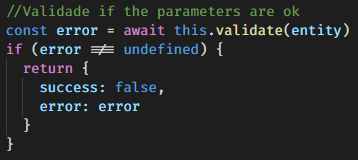
\includegraphics[scale=1.60]{./Figuras/code/server/controller-class-validator.png}
	\end{center}
	\legend{Fonte: os autores (2020)}
\end{figure}




\subsection{Middleware: Validação do JWT}


A figura \ref{code_server_class-validate} mostra a validação do token e a estratégia de renovação do token enviado. O middleware resgata o token JWT do header da requisição e aplica a regra da biblioteca jsonwebtoken para verificar se o JWT está com uma assinatura válida conforme a palavra-passe utilizada.
Caso a validação do JWT informado falhe, seja por não estar com a assinatura válida da aplicação ou por ter expirado o tempo da utilização, retorna um erro para a API informando que o token não é válido.
Caso a validação passe, o token é regerado com expiração renovada para 5 horas e é adicionado ao header da resposta.
Lembrando que, o token pode ser obtido através da rota de Login.

\begin{figure}[htb]
	\caption{\label{code_server_middleware}Middleware: Validação do JWT}
	\begin{center}
		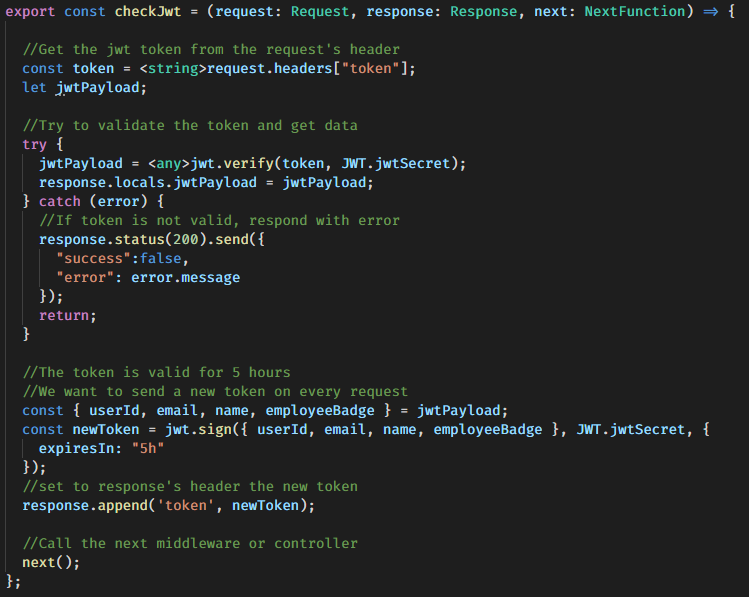
\includegraphics[scale=0.80]{./Figuras/code/server/middleware.png}
	\end{center}
	\legend{Fonte: os autores (2020)}
\end{figure}



\newpage
\subsection{TypeOrm: Query as Function}

A figura \ref{code_server_typeorm-query-as-function} mostra interação com o banco de dados montada pela ORM e disponibilizada como função. São funções montadas para buscar registros do banco de dados, temos a função chamada \textit{all}, esta faz a busca geral dos dados de uma tabela específica no banco de dados. Em contrapartida a função \textit{one} busca somente os dados de um filtro específico.

\begin{figure}[htb]
	\caption{\label{code_server_typeorm-query-as-function}TypeOrm: Query as Function}
	\begin{center}
		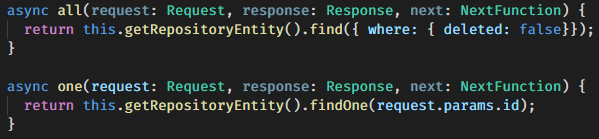
\includegraphics[scale=1.00]{./Figuras/code/server/typeorm-query-as-function.png}
	\end{center}
	\legend{Fonte: os autores (2020)}
\end{figure}



\subsection{Estratégia de Exclusão de Dados}

A figura \ref{code_server_delete-strategy} mostra a estratégia adotada para exclusão de resgistros, onde o registro não será realmente deletado, apenas irá alterar o atributo ''deleted'' para true. Desta maneira poderemos rapidamente desfazer uma exclusão errada e não teremos problemas com histórico apagado das entidades.

\begin{figure}[htb]
	\caption{\label{code_server_delete-strategy}Estratégia de Exclusão de Dados}
	\begin{center}
		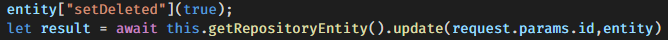
\includegraphics[scale=0.90]{./Figuras/code/server/delete-strategy.png}
	\end{center}
	\legend{Fonte: os autores (2020)}
\end{figure}
